\chapter{Entwurfsklassendiagramm}

Im folgenden Kapitel wird das Entwurfsklassendiagramm (EKD) genauer erklärt. Das EKD erweitert das Analyseklassendiagramm um Pakete, Methoden, Attribute und weitere Elemente, welche für die Umsetzung notwendig sind.

\section{Diagramm}

\begin{figure}[!ht]
    \centering
    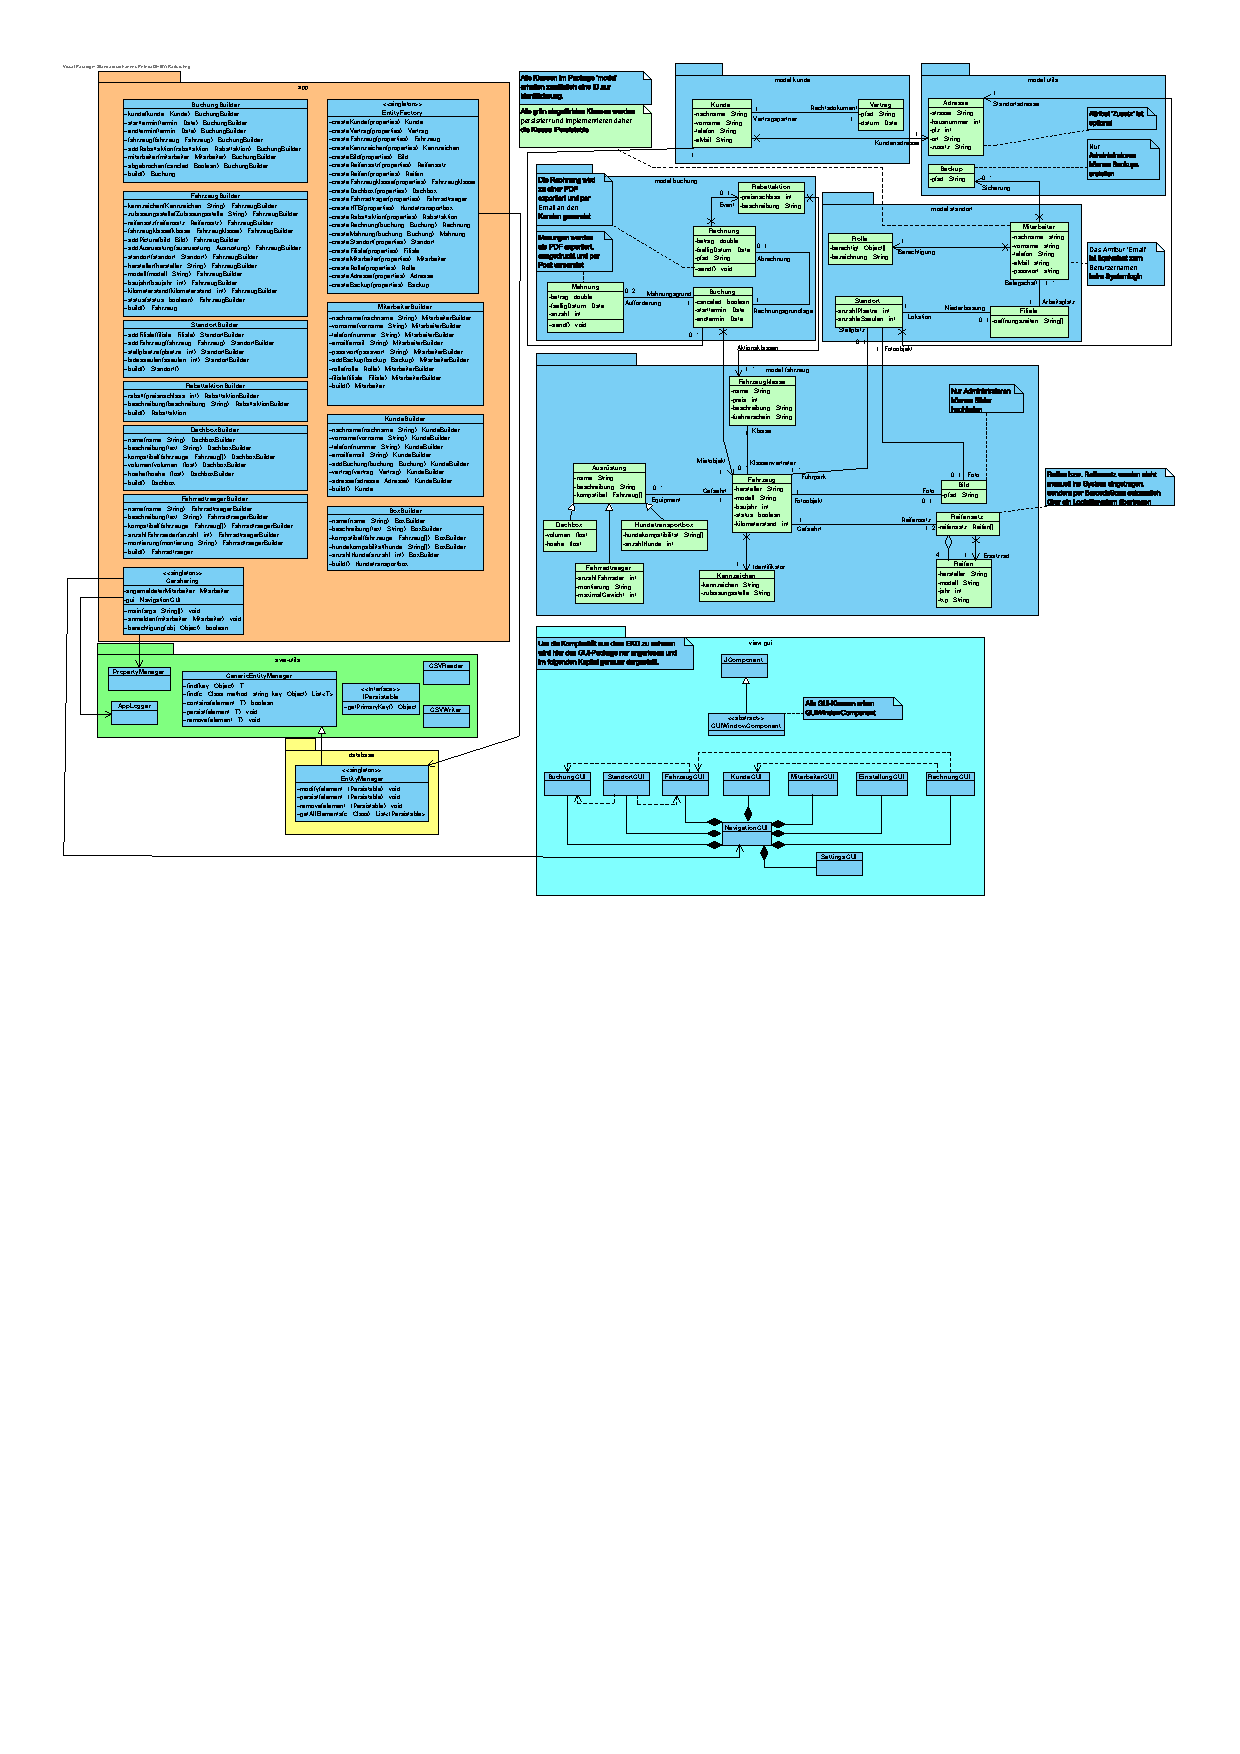
\includegraphics[width=\textwidth, trim = 0cm 13cm 0cm 0cm]{Bilder/Diagramme/Entwurfsklassendiagramm_v2.pdf}
    \caption{Aktivitätsdiagramm: Fahrzeug einem Standort zuordnen}
    \label{img:ekd}
\end{figure}

\newpage

\section{Pakete}

\subsection{model.buchung}

Dieses Paket enthält alle Klassen aus dem Analyseklassendiagramm, welche der Klasse 'Buchung' zugeordent werden können. Dazu gehören die Klassen 'Buchung', 'Rabattaktion', 'Rechnung' und 'Mahnung'. Damit auch die stornierten Buchungen noch eingesehen werden können, verfügt jede Buchung über ein Attribut, welches indiziert, ob die Buchung storniert wurde. Die Rabattaktion verfügt über ein Attribut für den prozentualen Preisnachlass. Die Rechnung ist durch Attribute für den Betrag der Rechnung und deren Fälligkeit definiert. Dazu gibt es eine Methode, um die Rechnung zum Kunden zu senden. Die Mahnung unterscheidet sich bezüglich der Attribute und methoden nicht von der Rechnung.

\subsection{model.fahrzeug}

Dieses Paket enthält alle Klassen, welche sich auf das Fahrzeug beziehen. Dazu gehören die Klassen 'Fahrzeug', 'Kennzeichen', 'Reifensatz', 'Reifen', 'Fahrzeugklasse', 'Bild' sowie 'Ausrüstung' und die Unterklassen der Ausrüstung ('Dachbox', 'Fahrradträger' und 'Hundetransportbox).
Das Fahrzeug besitzt Attribute, welche Auskunft über den Hersteller, das Baujahr und das Modell geben. Die Klasse 'Bild' speichert lediglich den Speicherort des Bildes. Die restlichen Klassen des Paketes verfügen jeweils über Attribute, um das Fahrzeug beziehnugsweise den dargestellten Bestandteil des Fahrzeuges genauer zu beschreiben. 

\subsection{model.kunde}

Dieses Paket enthält nur die Klasse 'Kunde' und die Klasse 'Vertrag' da dies Bereits alle Klassen sind, welche einen direkten Bezug zum Kunden haben.
Die Klasse 'Vertrag' enthält nur den Pfad, unter welchem der Vertrag gespeichert wurde. Die Klasse 'Kunde' enthält hingegen alle Informationen, welche für die Kontaktierung des Kunden notwendig sind.

\subsection{model.standort}

Dieses Paket enthält alle Klassen, welche einen Standort sowie dessen Mitarbeiter darstellen. Dazu gehören neben der Klasse 'Standort' auch die Klassen 'Filiale', 'Mitarbeiter' und 'Rolle'. Die Rolle definiert dabei auf welche Objekte ein Mitarbeiter zugreifen darf. Sowohl für die Standorte als auch für die Filialen wird für statistische Erhebungen die Anzahl der Mitarbeiter angegeben. Der Mitarbeiter wird ähnlich wie der Kunde hauptsächlich durch Kontaktinformationen dargestellt. Jedoch wird außerdem noch das Gehalt des Mitarbeiters gespeichert.

\subsection{model.utils}

In diesem Paket befinden sich Klassen, welche von verschiedenen anderen Klassen verwendet werden. Dazu gehört neben der Klasse 'Adresse' auch die Klasse 'Backup'.

\subsection{app}

Hier befindet sich zum einen die zentrale Klasse 'Carsharing', welche die Main-Methode für das Starten der Anwendung beinhaltet. Diese Klasse wird als Singleton implementiert. Zum anderen befindet sich hier die 'EntityFactory' und der 'BuchungBuilder', welche für das Erzeugen von Instanzen der Klassen aus den Model-Paketen, welche in der Datenbasis gespeichert werden. Für die Buchungen wird extra ein Builder implementiert, da es sich hierbei um eine besonders komplexe Klasse handelt. 

\subsection{swe-utils}

Dieses Paket enthält eigentlich noch wesentlich mehr Klassen, welche jedoch nicht mit dargestellt werden, da sie für die Anwendung irrelevant sind. Die enthalten Klassen beinhalten den 'CSVReader' und 'CSVWriter', welche im EntityManager für das Speichern der Daten eingesetzt werden. Für diese Persistierung der Daten ist das Interface 'IPersistable' enthalten. Außerdem befindet sich hier auch der 'PropertyManager' und der 'AppLogger'.

\subsection{database}
Dieses Paket beinhaltet nur eine Klasse. Dabei handelt es sich um den generischen 'EntityManager', welcher von der Klasse 'GenericEntityManager' aus dem Paket 'swe-utils' erbt. Diese Klasse wird als Singleton implementiert und ist für die Verwaltung der Entitäten verantwortlich.

\subsection{gui}
Dieses Paket beinhaltet alle Klassen, welche die Benutzeroberfläche betreffen. Dazu gehören neben einer Vielzahl von Klassen, welche auf 'GUI' enden auch die abstrakte Klasse 'GUIComponent' und die Klasse 'JComponent'. 'GUIComponent' erbt hierbei von 'JComponent' und alle auf 'GUI' endenden Klassen erben von 'GUIComponent'. Diese Klassen, welche auf 'GUI' enden stellen die einzelnen Ansichten der Anwendung dar. Im Sinne der Übersichtlichkeit wurde in diesem Diagramm auf die Detailtiefe bezüglich der Benutzeroberfläche verzichtet. Diese wird im nächsten Kapitel ab Seite \pageref{chapter:gui} genauer beschrieben.

\section{Entwurfsmuster}
Für die Implementierung der Carsharingsoftware verwenden wir verschiedene Entwurfsmuster, welche das Auftreten von Problemen verhindern sollen. Solche Entwurfsmuster sind wiederverwendbare Schablonen zur Problemlösung. Im folgenden Abschnitt werden die verwendeten Entwurfsmuster genauer erläutert und erklärt, wie diese für die Implementierung eingesetzt werden. 

\subsection{EntityManager}
Bezüglich des EntityManagers wurde sich dafür entschieden eine generische Klasse zu implementieren, welche alle gespeicherten Entitäten verwaltet. Dies hat den Vorteil, dass die Verwaltung der Entitäten sehr simpel dargestellt und Implementiert werden kann.

\subsection{Builder}
Für das Erstellen von komplexeren Klassen setzen wir in unserem Entwurf sogenannte Builder ein. Zu diesen Klassen gehören die Buchung, das Fahrzeug, der Standort sowie der Mitarbeiter. Durch den Builder wird ein schrittweises Erstellen von Instanzen dieser Objekte ermöglicht, wodurch die Erstellung dieser Objekte deutlich vereinfacht wird.

\subsection{EntityFactory}
Die EntityFactory wird verwendet, um Instanzen einzelner Klassen zu erstellen. Dazu verfügt die EntityFactory für jede Klasse, für welche eine Instanz erzeugt werden soll, über eine Methode, welche nach der Persistierung des Objektes mithilfe des EntityManagers eine Instanz zurückgibt. Um solche Insatnzen zu erstellen, müssen den Methoden verschiedene Parameter übergeben werden. Diese Parameter werden im Diagramm zur Vereinfachung als 'properties' dargestellt.

\subsection{Singleton}
Ein Singleton stellt sicher, dass es zu einer Klasse nur genau ein einziges Objekt gibt. Diese Singletons werden in unserem Entwurf an verschiedenen Stellen eingesetzt. Bei diesen Stellen handelt es sich um die Klasse 'Carsharing', den EntityManager und die EntityFactory. Mit der Verwendung dieses Entwurfsmusters wird die Verhinderung des Auftretens von Dateninkonsistenzen beabsichtigt.

\subsection{Beobachter}
Mit Beobachtern kann auf die Veränderung von Objekten reagiert werden. Solche Beobachter wurden in unserem Entwurf lediglich passiv implementiert. Das heißt, dass die Beobachter nicht aktiv den Zustand eines konkreten Objektes abfragen, sondern nur dann benachrichtigt werden , wenn Änderungen aufgetreten sind. Dadurch ergibt sich eine größere Vielfalt der Abstraktionsmöglichkeiten und die Wiederverwendbarkeit von einzelnen Komponenten.

\subsection{Kompositum}
Das Kompositum wird genutzt um Teil-Ganzes-Hierachien darzustellen. In unserem Entwurfsklassendiagramm wird dies zum einem bei der Modellierung des Reifensatzes eines Fahrzeuges und zum anderen auch bei der Modellierung der Benutzeroberfläche genutzt. Ein Reifensatz besteht hierbei aus vier oder fünf Reifen, je nachdem, ob ein Ersatzrad vorhanden ist und bei der Benutzeroberfläche sind die Unteransichten ein Teil der Hauptansicht.